%
%  intro.tex
%
%  Created by Drew Conway on 2011-01-26
% 
%
\documentclass[xcolor=dvipsnames, 9pt]{beamer}

\usepackage{amssymb}
\usepackage{amsfonts}
\usepackage{amsmath}
\usepackage{hyperref}
\usepackage{natbib}
\usepackage{color}
\usepackage{pdfsync}
\usepackage{chancery}
\usepackage{movie15}
\usepackage{pgfpages}
\usepackage{fancyvrb}
\usepackage{colortbl}
\usepackage{multirow}

\usepackage{graphicx}
\graphicspath{{../../images/figures/}{../../images/logos/}{../../images/graphs/}/}

\usepackage{beamerthemesplit}
\usetheme{Copenhagen}
\definecolor{title}{RGB}{128,148,182}
\usecolortheme[named=title]{structure} 
\setbeamertemplate{headline}{}
\setbeamertemplate{navigation symbols}{}
\setbeamertemplate{itemize items}[triangle]
\setbeamertemplate{enumerate items}[default]
\setbeamertemplate{footline}[page number]{}
%\setbeameroption{show notes on second screen}


\usepackage{listings}
%\usepackage{listings,arev}
\definecolor{keywords}{RGB}{128,148,182}
\definecolor{comments}{RGB}{60,179,113}
\lstset{numbers=left,
        showstringspaces=false,
        numberstyle=\tiny,
        %frame=leftline,
        numbersep=4.5pt,
  keywordstyle=\color{keywords}\bfseries,
  commentstyle=\color{YellowOrange}\emph
}

\newenvironment{code}{\begin{semiverbatim} \begin{footnotesize}}
{\end{footnotesize}\end{semiverbatim}}


\newcommand{\R}{\mathbb{R}}
\renewcommand{\d}{\mathsf{d}}
\newcommand{\dd}{\partial}
\newcommand{\E}{\mathsf{E}}
\newcommand{\bb}{\mathbf}

\title{Visualization Basics}
\author{Joseph Adler, Drew Conway, Jake Hofman, Hilary Mason}
\date{February 1, 2011}

\begin{document} 
    
\begin{frame}[plain]
  \titlepage 

  \tiny
  \href{http://creativecommons.org/licenses/by-sa/3.0/us/}{
\includegraphics[width=1cm]{ccbysa}}

  Creative Commons Attribution-Share Alike 3.0
\end{frame}

\section{Data Visualization Introduction} % (fold)
\label{sec:visualization}

\subsection{What data visualization should do} % (fold)
\label{sub:what_data_visualization_should_do}

{
\setbeamercolor{background canvas}{bg=}
\usebackgroundtemplate{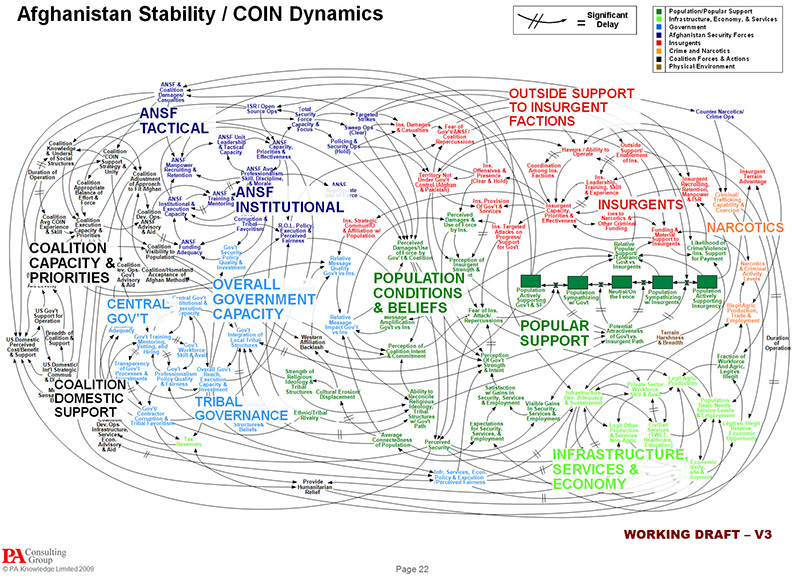
\includegraphics[width=\paperwidth,
height=\paperheight]{Afgan-orig-med.jpg}}
\begin{frame}[fragile]
    \frametitle{}
    \vspace{4cm}
    \begin{center}
        \begin{minipage}{5cm}
        \uncover<2->{\begin{varblock}[6cm]{What data visualization should do?}
            \begin{enumerate}
                \uncover<3->{\item Make complex ideas \textbf{simple}}
                \uncover<4->{\item Extract \textbf{small} info from big data}
                \uncover<5->{\item Present \textbf{truth}, not deceive}
            \end{enumerate}
        \end{varblock}}
    \end{minipage}
    \end{center}
\end{frame}
}

\begin{frame}[fragile]
    \frametitle{Make complex ideas \textbf{simple}}
    \begin{center}
        \only<1>{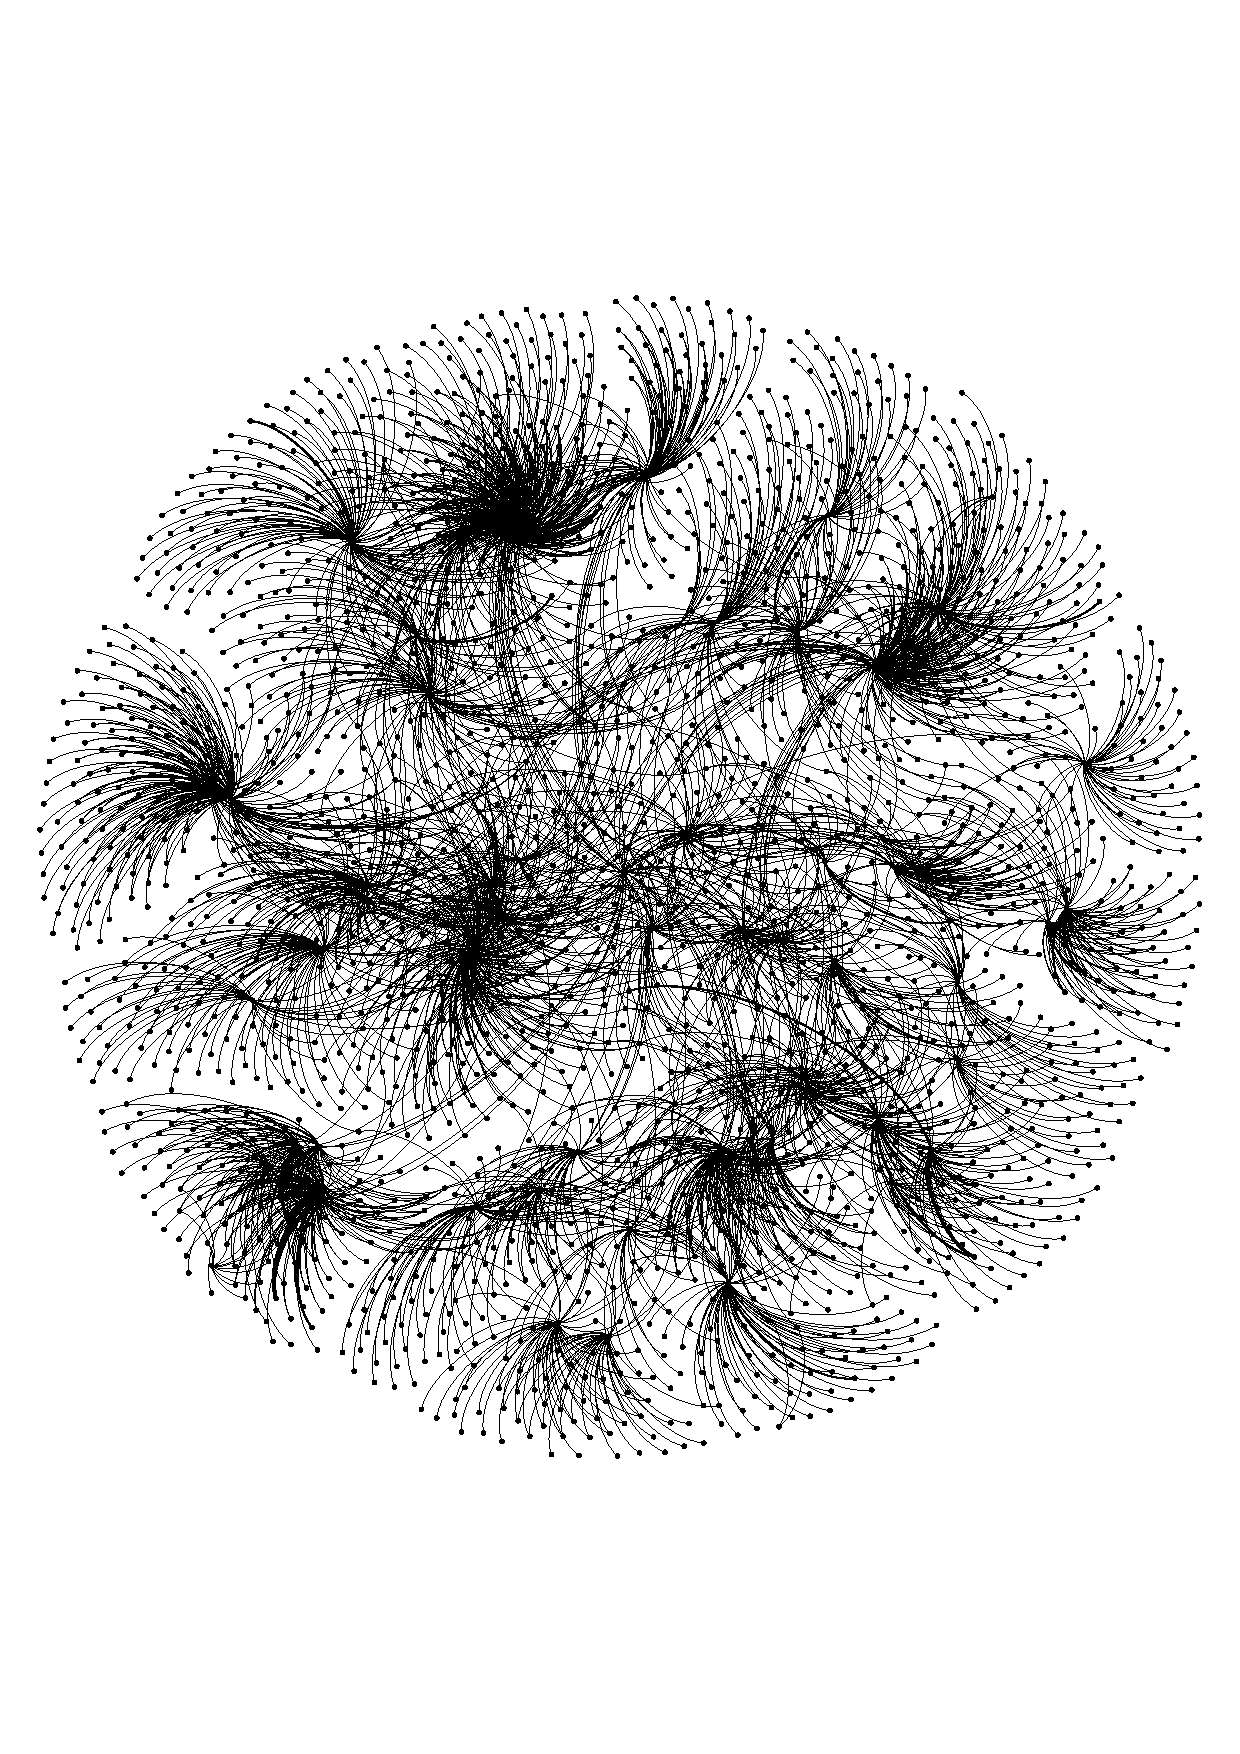
\includegraphics[height=8cm,clip,trim=0cm 5cm 0cm 5cm]{full_ibes_weighted_mc}}
        \only<2>{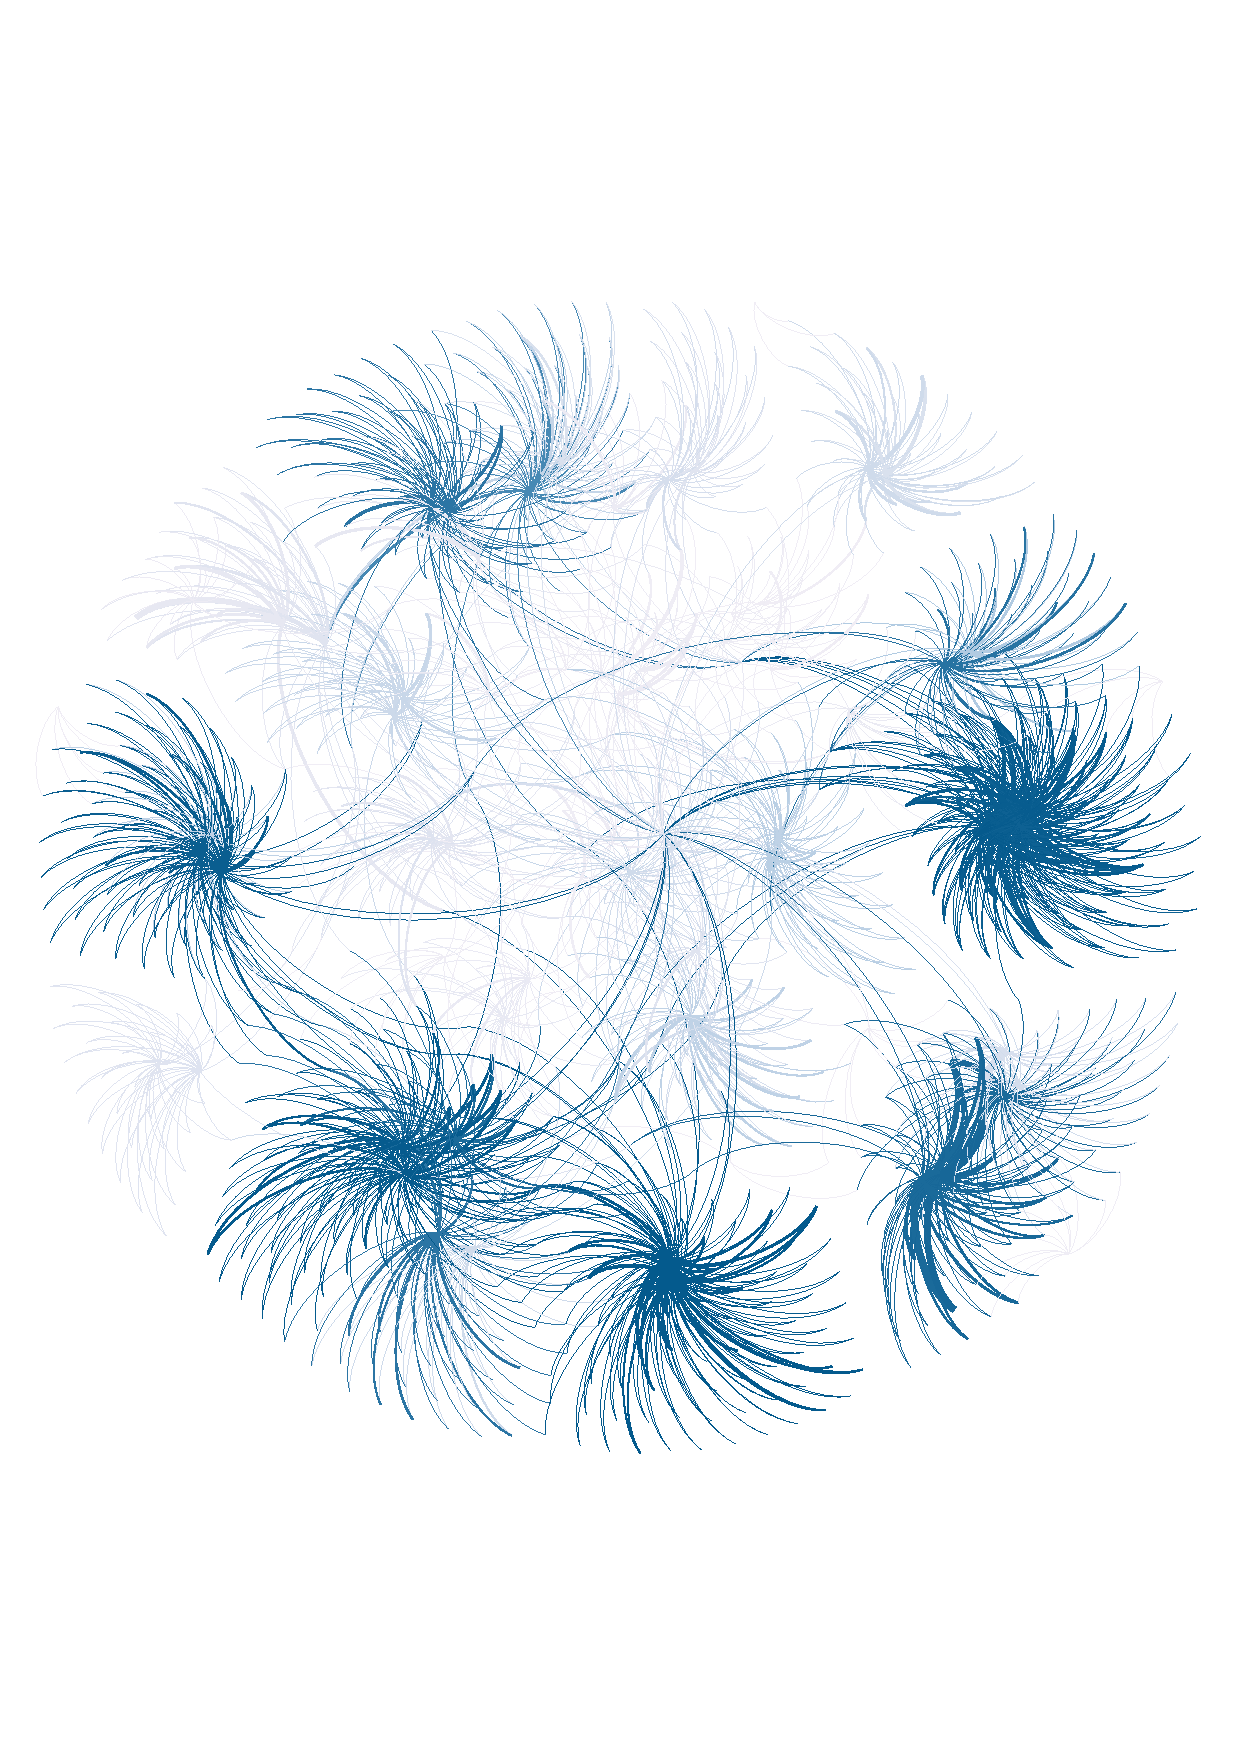
\includegraphics[height=8cm,clip,trim=0cm 5cm 0cm 5cm]{full_ibes_weighted_mc_2c_reduce.pdf}}
    \end{center}
\end{frame}

\begin{frame}[fragile]
    \frametitle{Good example of complexity reduction}
    \begin{center}
        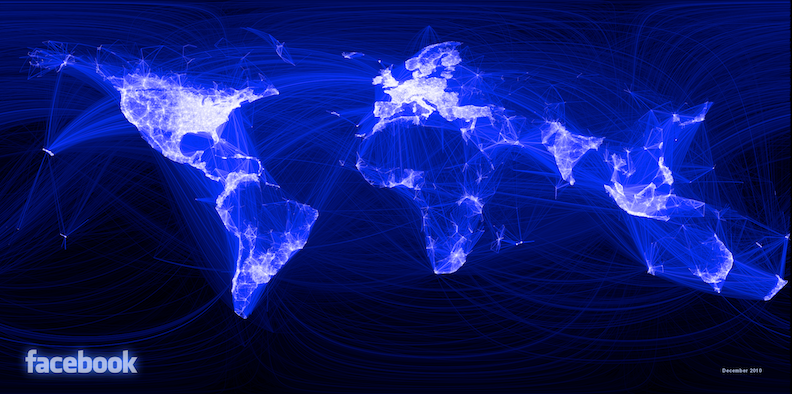
\includegraphics[width=11cm]{facebook_map_reduce.png}
    \end{center}
\end{frame}


\begin{frame}[fragile]
    \frametitle{Extract \textbf{small} info from big data}
    \begin{center}
        \only<1>{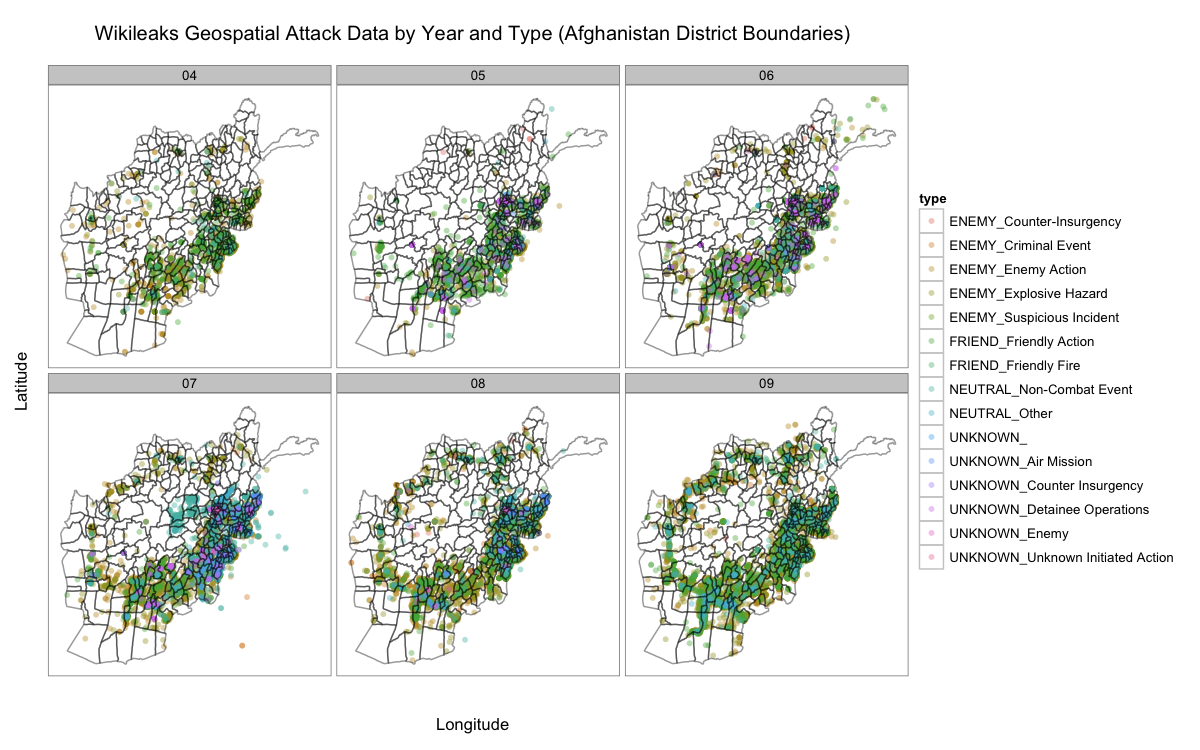
\includegraphics[width=11cm]{events_by_year_map.png}}
        \only<2>{\includegraphics[width=10cm]{ied_by_year.pdf}}
    \end{center}
\end{frame}

\begin{frame}[fragile]
    \frametitle{Present \textbf{truth}, do not deceive}
    \begin{center}
        \only<1>{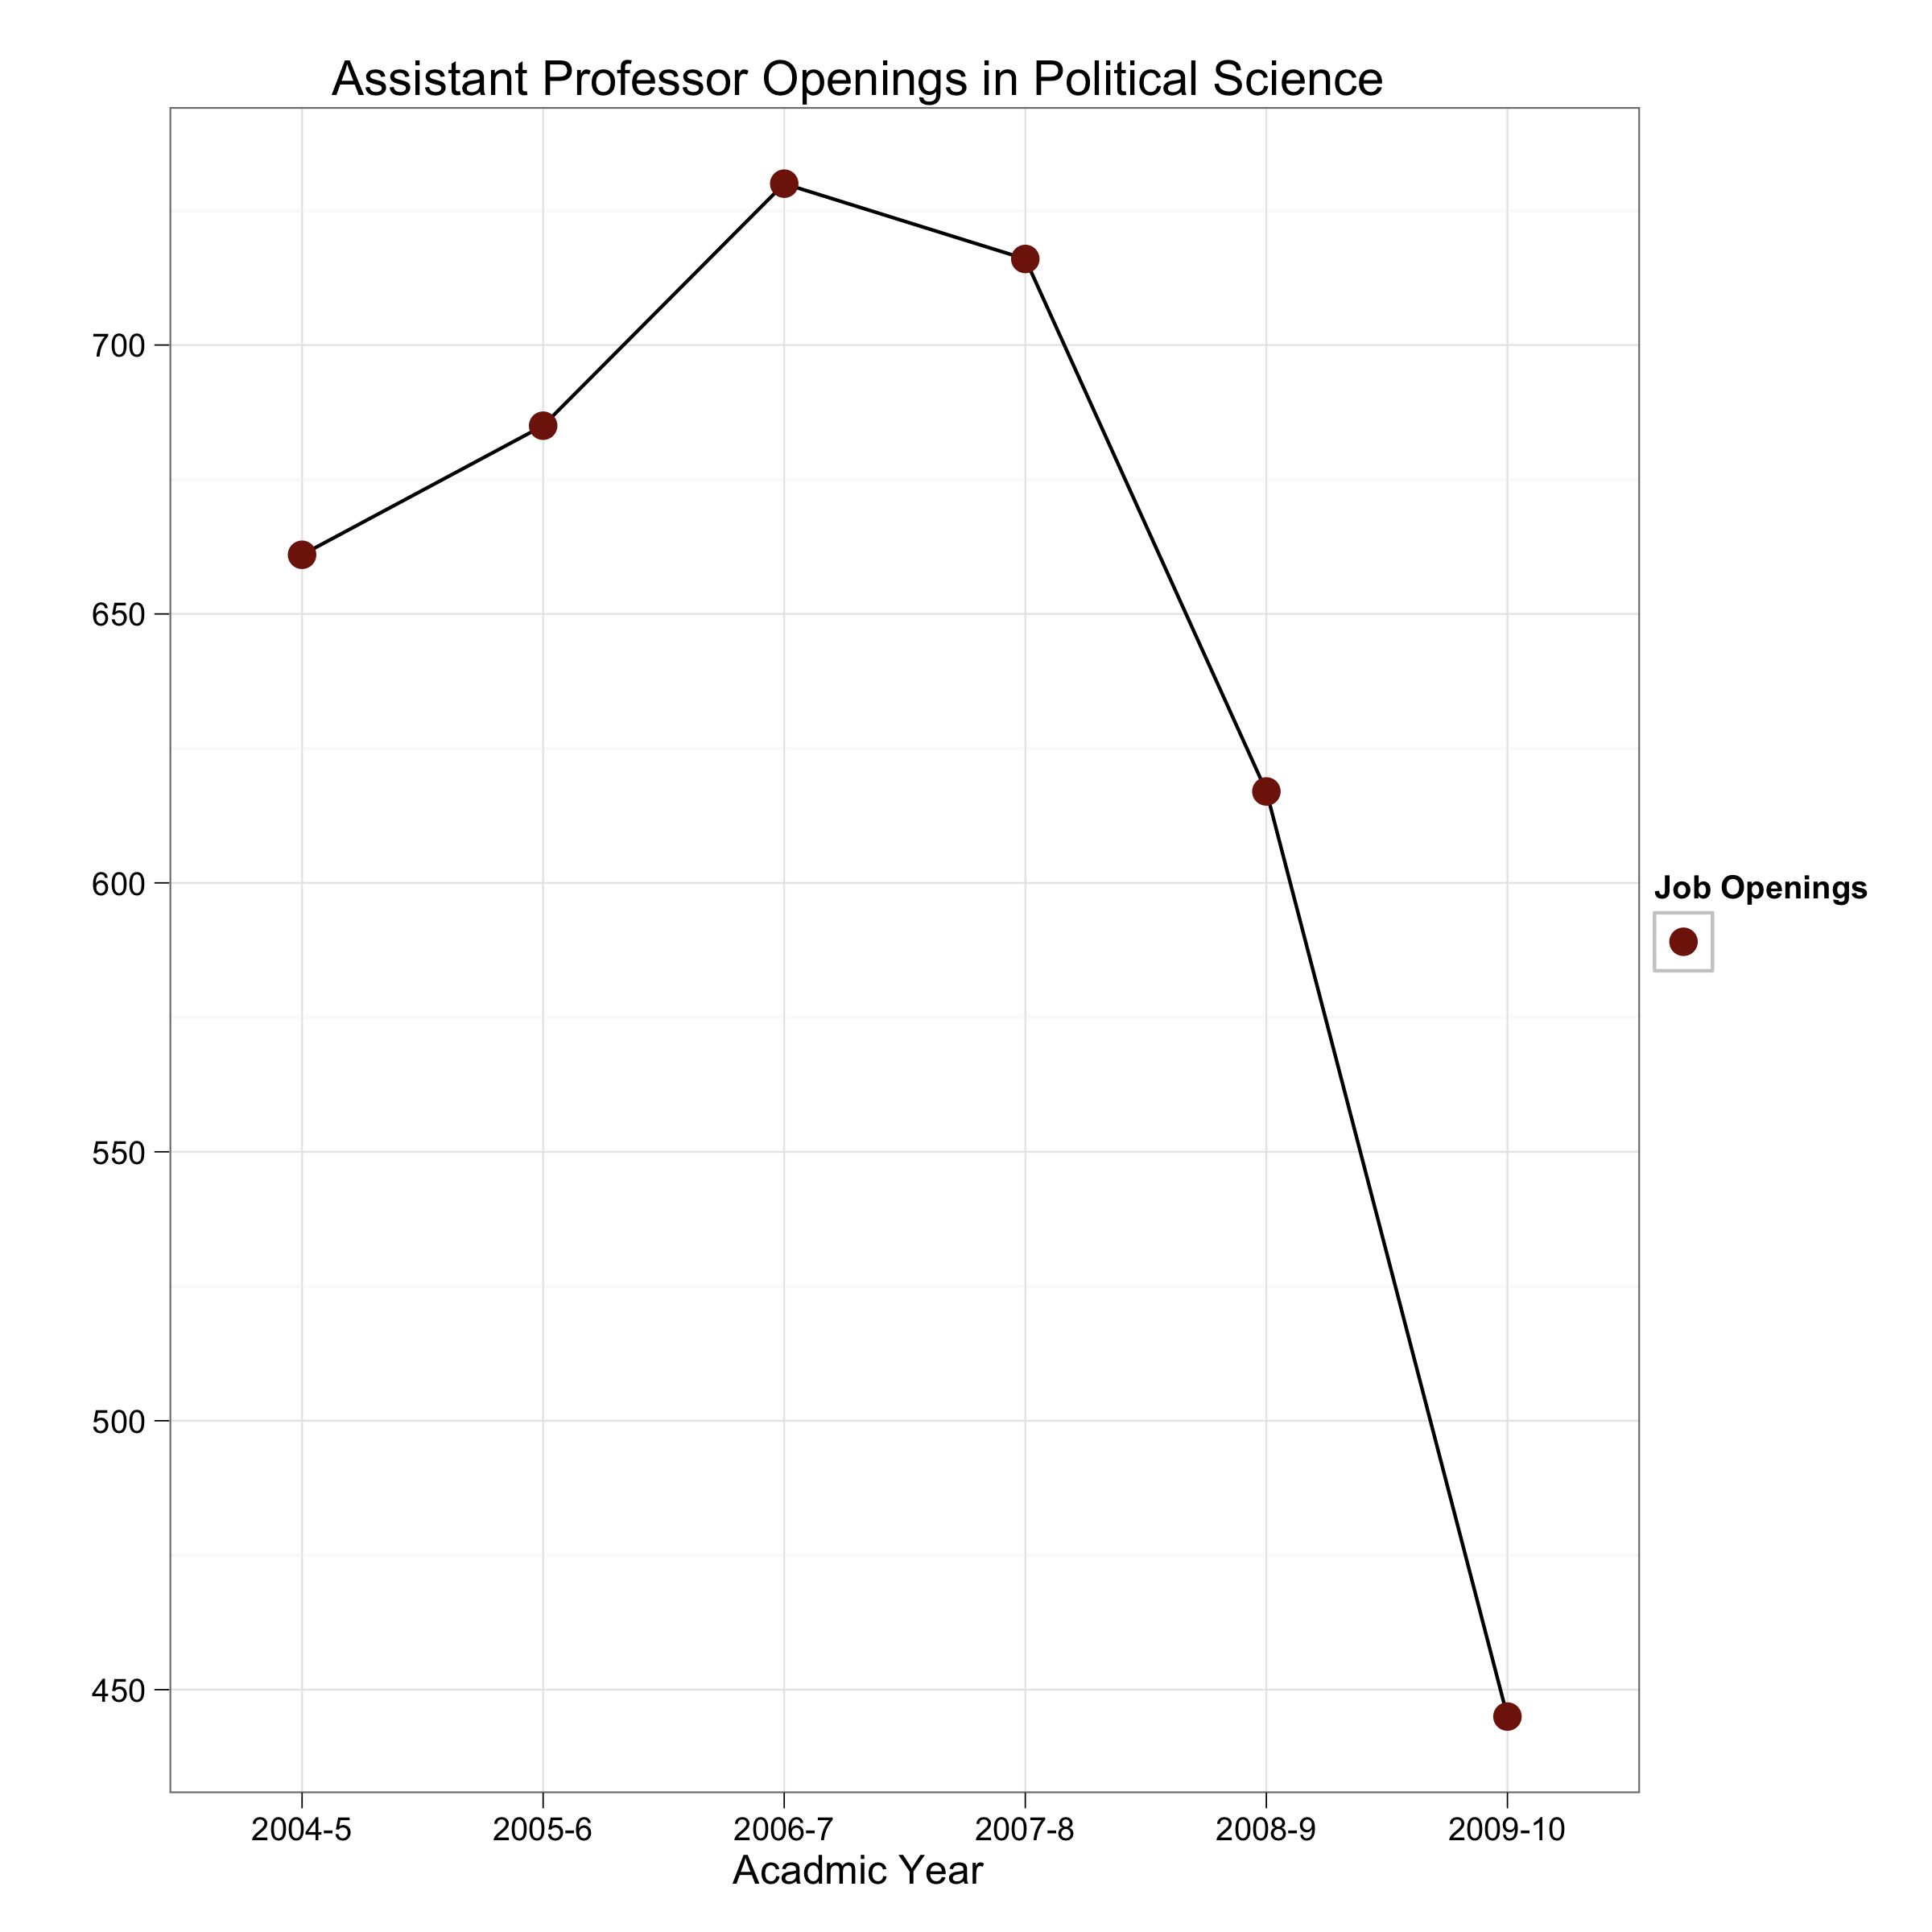
\includegraphics[height=8cm,width=10cm]{poli_sci1.png}}
        \only<2>{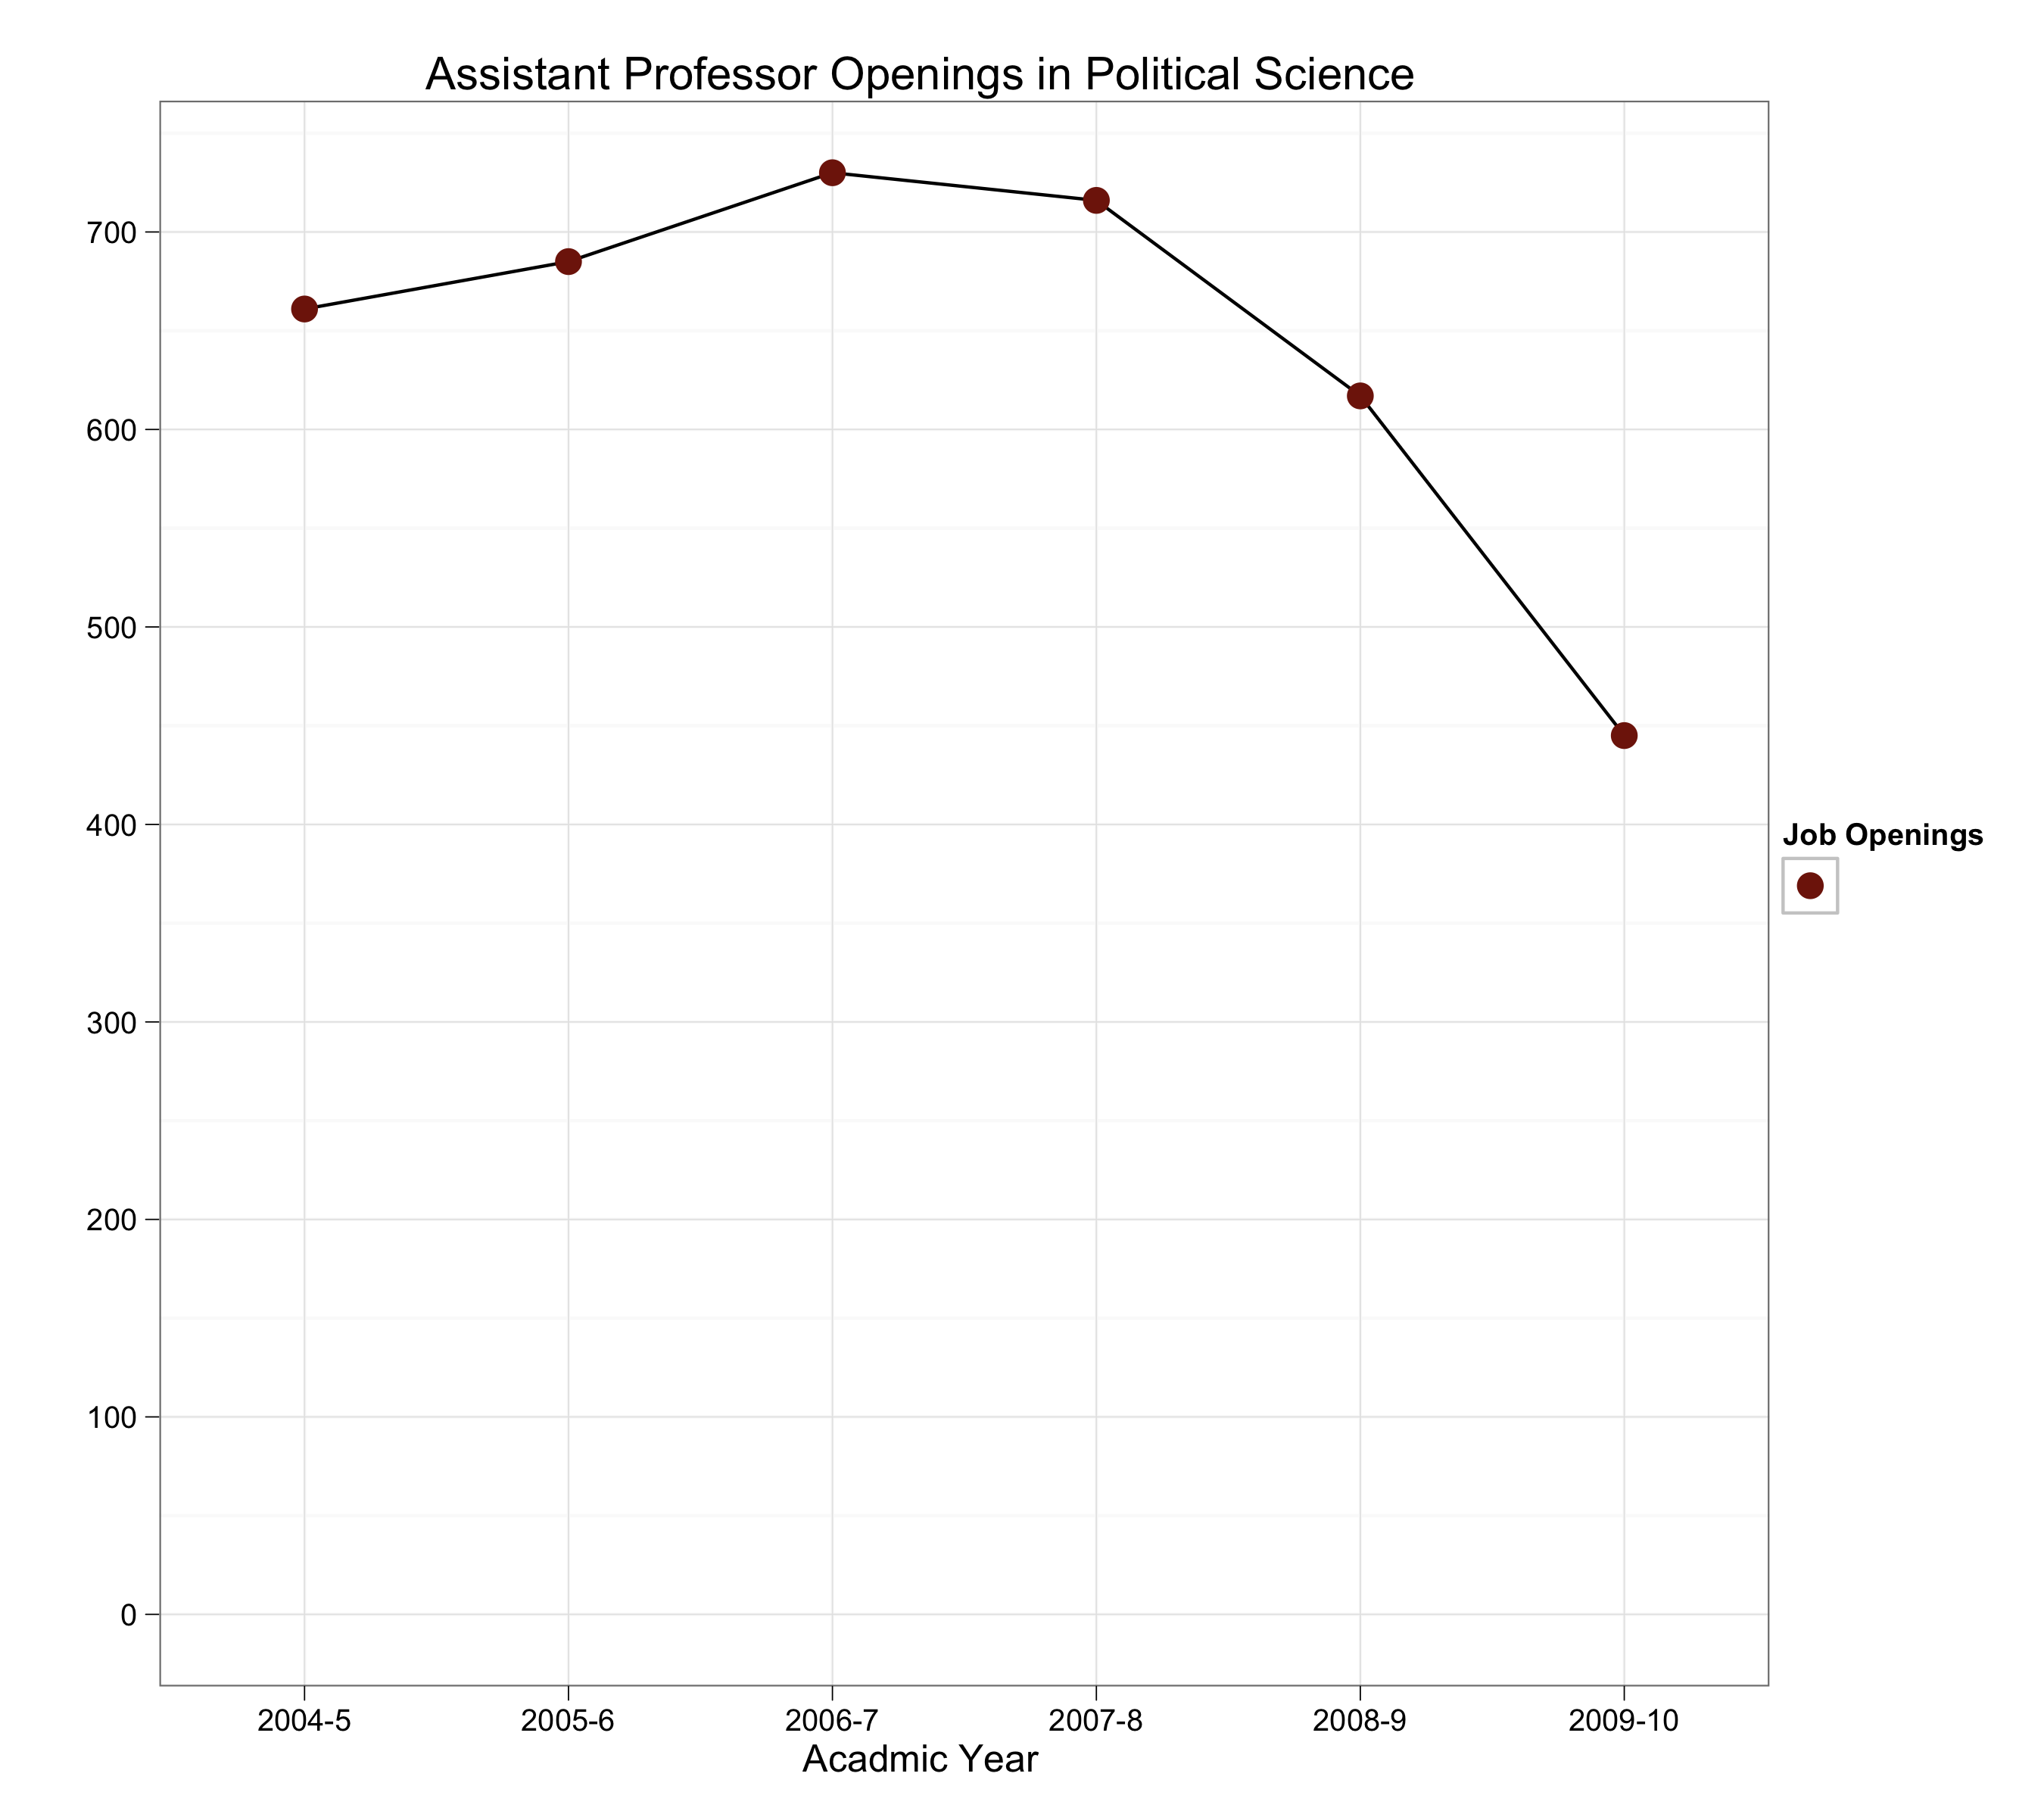
\includegraphics[height=8cm,width=10cm]{poli_sci2.png}}
    \end{center}
\end{frame}

% subsection what_data_visualization_should_do (end)

\subsection{Data visualization tools} % (fold)
\label{sub:data_visualization_tools}

\begin{frame}[fragile]
    \frametitle{Commercial data visualization tools}
    Data visualization is very popular...
    \begin{center}
        
\includegraphics[width=10cm]{google_data_viz_count.png}
        \uncover<2->{\begin{block}{Strata $\heartsuit$'s visualization!}
\tiny{\begin{code}
\$ wget -O strata.htm http://strataconf.com/strata2011/public/schedule/full

\$ tr -cs `A-Za-z' `$\backslash$n' < strata.html | grep -c ``visual''

\alert{24}
\end{code}}
        \end{block}}
    \end{center}
    \uncover<3->{\begin{columns}[c]
        \column{.33\textwidth}
        
\includegraphics[width=3cm]{juice_white_small.jpg} \\ \vspace{4mm}
        
\includegraphics[width=3cm]{tableau_logo.png} \\ \vspace{4mm}
        
\includegraphics[width=3cm]{periscopic.png}
        \column{.33\textwidth}
        
\includegraphics[width=3cm]{gooddata.png} \\ \vspace{4mm}
        
\includegraphics[width=3cm]{google.png} \\ \vspace{4mm}
        
\includegraphics[width=3cm]{digital_reasoning.png}
        \column{.33\textwidth}
        
\includegraphics[width=3cm]{readwriteweb-logo.png} \\ \vspace{4mm}
        
\includegraphics[width=3cm]{200px-The_New_York_Times_Company_logo.png} \\ \vspace{4mm}
        
\includegraphics[width=3cm]{the-guardian-logo.jpg}
    \end{columns}}
\end{frame}

\begin{frame}[fragile]
    \frametitle{Open-source visualization tools}
    For this tutorial we will not be using any commercial tools
    \begin{itemize}
        \item Instead utilizing \textbf{only open-source tools}
    \end{itemize}
    \uncover<2->{There are many tools at our disposal
    \begin{itemize}
        \item Here we will use \textbf{two premier scientific computing environments}
    \end{itemize}}
    \vspace{1cm}
    \uncover<2->{\begin{columns}
        \column{0.5\textwidth}
        \begin{center}
            
\includegraphics[width=6cm]{python-logo-master-v3-TM.png}
        \end{center}
        \column{0.5\textwidth}
        \begin{center}
            
\includegraphics[height=3cm]{200px-Rlogo.png}
        \end{center}
    \end{columns}}
\end{frame}

\begin{frame}[fragile]
    \frametitle{Python's scientific computing holy trinity}
    \begin{right}
        \uncover<9->{\hfill \textbf{\alert{$\searrow$}\hspace{2cm}\alert{$\swarrow$}}}
    \end{right}
    \begin{columns}
        \column{.33\textwidth}
        \begin{center}
            \href{http://www.scipy.org}{
\includegraphics[width=3cm]{Scipylogo.png}}
        \end{center}
        \uncover<2->{Python's primary library for \textbf{mathematical and statistical} computing. Containing sub-libs for
        \begin{itemize}
            \item Numeric optimization
            \item Clustering
            \item Linear algebra
            \item ..and many others
        \end{itemize}}
        \uncover<3->{The primary data type in \texttt{SciPy} is an array
        \begin{itemize}
            \item Data manipulation is similar to that of MATLAB
        \end{itemize}}
        \vspace{3mm}
        \column{.33\textwidth}
        \begin{center}
            \href{http://numpy.scipy.org/}{
\includegraphics[clip,trim=0mm 2mm 0mm 2mm,width=2.5cm]{NumPy_logo.png}}
        \end{center}
        \uncover<4->{\texttt{NumPy} is an extension of the \texttt{SciPy} data type to include \textbf{multidimensional arrays and matrices}
        \begin{itemize}
            \item Provides many functions for working on arrays and matrices
            \item Very useful for representing relational data
        \end{itemize}}
        \uncover<5->{Both \texttt{SciPy} and \texttt{NumPy} rely on the C library \texttt{LAPACK} for very fast implementation}
        \column{.33\textwidth}
        \begin{center}
            \href{http://matplotlib.sourceforge.net/}{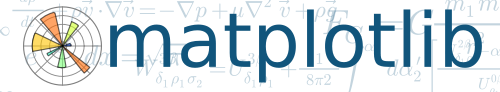
\includegraphics[width=3cm]{500px-Matplotlib_logo.png}}
        \end{center}
        \uncover<6->{\texttt{matplotlib} is \textbf{primary plotting library in Python}
        \begin{itemize}
            \item Supports 2- and 3-D plotting
            \item API allows embedding in apps
        \end{itemize}}
        \uncover<7->{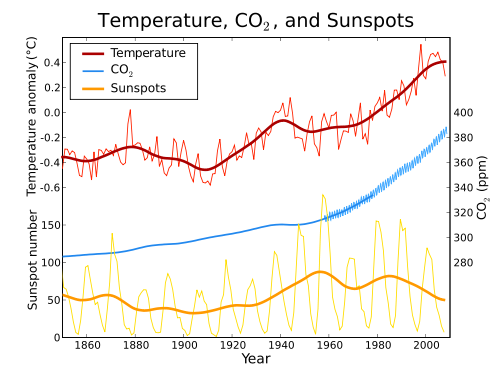
\includegraphics[width=2cm]{500px-Temp-sunspot-co2.png}
        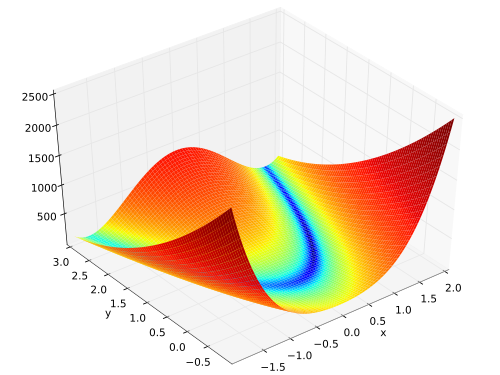
\includegraphics[width=2cm]{500px-Rosenbrock_function.png}}\\
        \uncover<8->{All graphics are highly customizable and professional publication ready}
    \end{columns}
    \vspace{1mm}
\end{frame}

\begin{frame}[fragile]
    \frametitle{Data visualization in in R}
    \uncover<10->{\hfill \textbf{\alert{$\searrow$}\hspace{1cm}\alert{$\swarrow$}\hspace{1.55cm}}}
    \begin{columns}
        \column{0.33\textwidth}
            \Large{\underline{The \texttt{R} Language}} \\ \vspace{2mm}
            \uncover<2->{\footnotesize{``freely available language and environment for statistical computing and graphics...''}} \\ \vspace{2mm}
            \normalsize
            \uncover<3->{CRAN
            \begin{itemize}
                \item Massive library of specialized packages
                \item 2,775 available
            \end{itemize}}
           \uncover<4->{R Task Views
            \begin{itemize}
                \item 28 development areas
                \item Bayesian, ML, NLP, \textbf{Graphics}
            \end{itemize}}
            \uncover<5->{Two popular visualization packages
            \begin{itemize}
                \item \texttt{lattice}
                \item \texttt{ggplot2}
            \end{itemize}}
        \column{0.33\textwidth}
            \Large{\texttt{\underline{lattice}}} \\ \vspace{2mm}
            \normalsize
            \uncover<6->{Developed by Deepayan Sarkar \\ 
            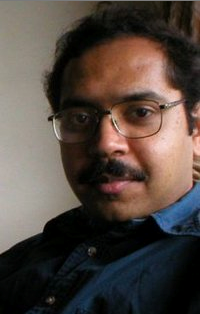
\includegraphics[height=2.5cm]{Deepayan-Sarkar.png}
            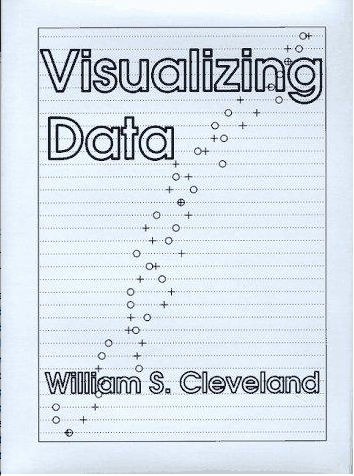
\includegraphics[height=2.5cm]{cleveland.png} \\
            \uncover<7->{\begin{itemize}}
                \item Implementation of Trellis graphics
            \end{itemize}
            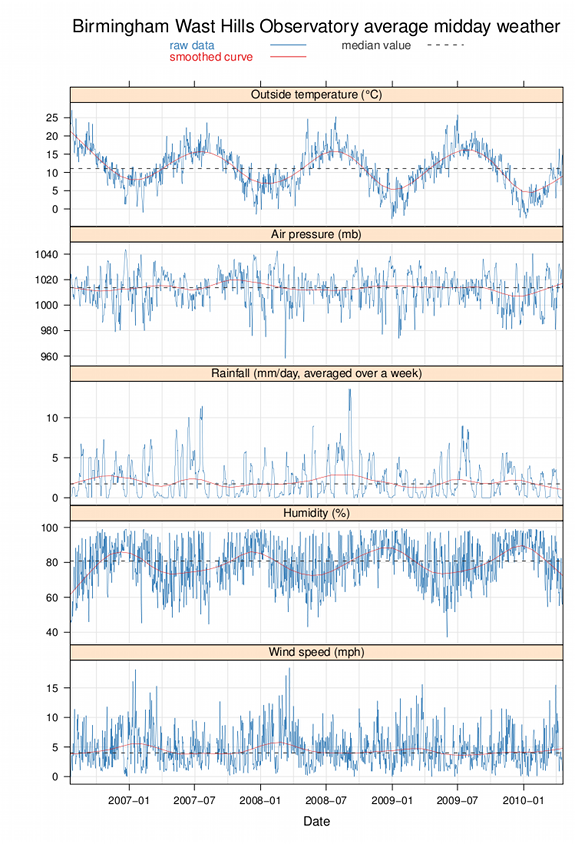
\includegraphics[height=2.2cm]{midday_weather_profiles.png}
            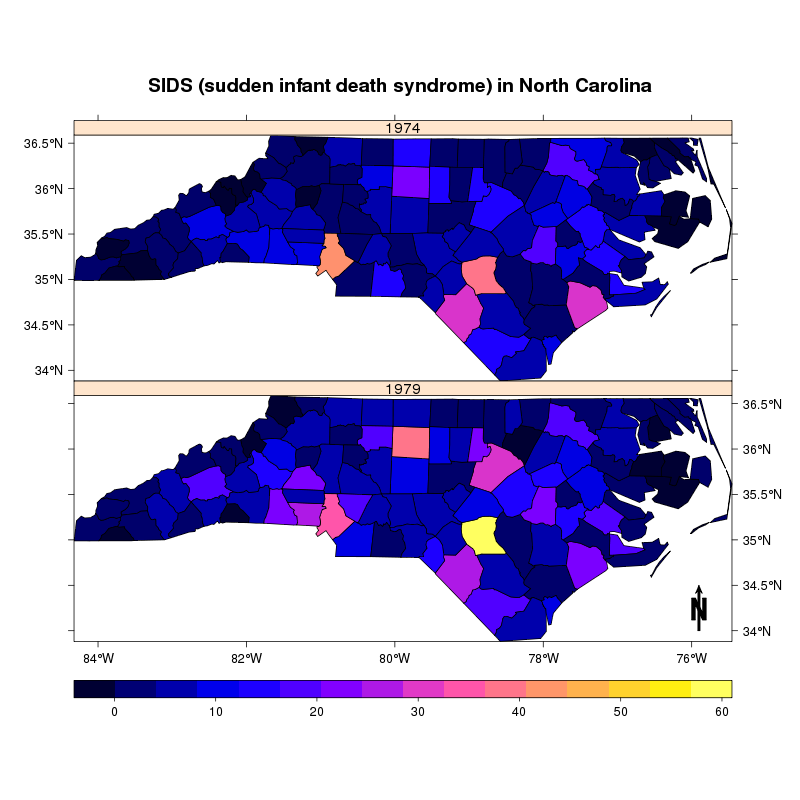
\includegraphics[height=2.2cm]{fig09.png}}
        \column{0.33\textwidth}
            \Large{\texttt{\underline{ggplot2}}} \\ \vspace{2mm}
            \normalsize
            \uncover<8->{Developed by Hadley Wickham \\
            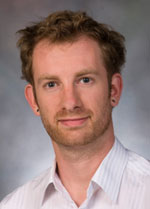
\includegraphics[height=2.5cm]{wickham.jpg}
            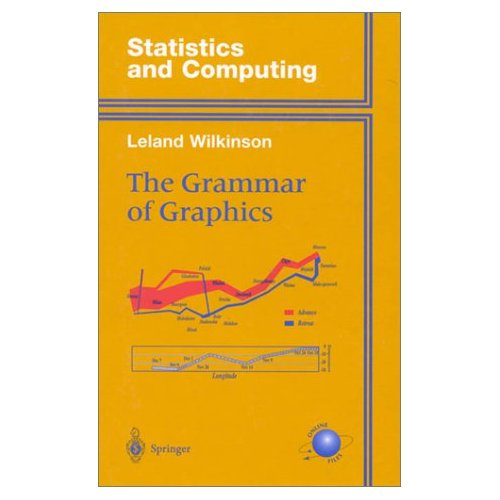
\includegraphics[height=2.5cm,clip,trim=2mm 0mm 2mm 0mm]{wilkinson.jpg} \\}
            \uncover<9->{\begin{itemize}
                \item Visualizations are ``grammatical layers''
            \end{itemize}
           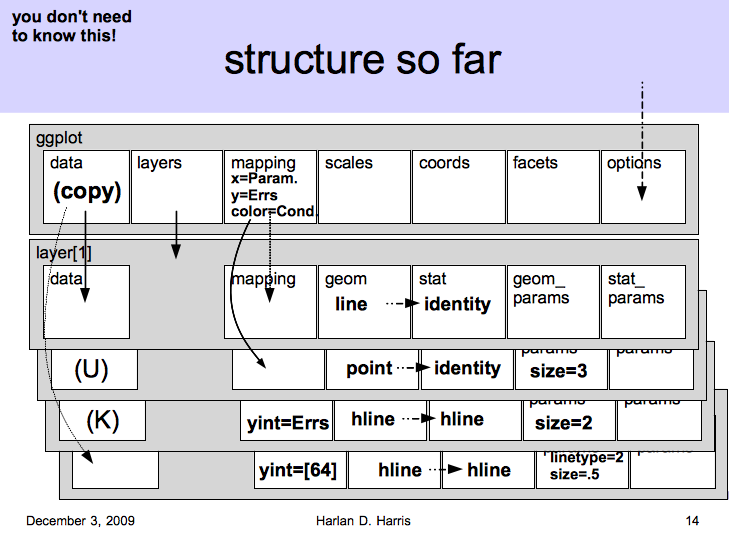
\includegraphics[width=3cm]{ggplot2_layers.png}\\ \hfill\tiny{Image source: Harlan Harris}}
    \end{columns}
\end{frame}

% subsection data_visualization_tools (end)

\subsection{My first visualization} % (fold)
\label{sub:my_first_visualization}

\begin{frame}[fragile]
    \frametitle{Creating a simple visualization}
    As an introduction to each environment we will make the same plot in both \texttt{matplotlib} and \texttt{ggplot2} \\ 
    \vspace{2mm}
    \uncover<2->{To begin, we'll generate canonical data and visualize it
    \begin{itemize}
        \item Histogram of 10,000 randomly generated numbers from a \textbf{standard Normal distribution}
        \item $\mu = 0$, $\sigma = 1$
        \item Then, overlay Normal density function to observe ``fit''\footnote{Image source: \url{http://mathworld.wolfram.com/NormalDistribution.html}}
    \end{itemize}}
    \uncover<3->{\begin{center}
        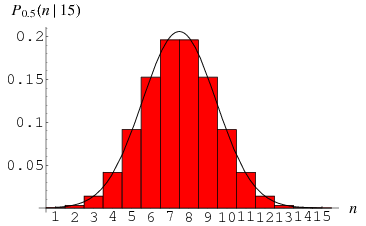
\includegraphics[width=5cm]{BinomialGaussian_1000.png}
    \end{center}}
    \uncover<4->{We'll start by working in Python with \texttt{matplotlib}...}
\end{frame}

\begin{frame}[fragile]
    \frametitle{My first \texttt{matplotlib} visualization: 1/3}
    Out first steps are to load the libraries and generate data
    \begin{block}{\texttt{matplotlib} and the normal distribution}
        \begin{lstlisting}[language=Python]
>>> import matplotlib.pylab as plt
>>> from scipy.stats import norm
        \end{lstlisting}
    \end{block}
    \begin{block}{Generate 10,000 random draws from a normal}
        \begin{lstlisting}[language=Python]
>>> random_normal = norm.rvs(0,1,size=10000)
        \end{lstlisting}
    \end{block}
    \begin{block}{Create a \texttt{figure} to draw to}
        \begin{lstlisting}[language=Python]
>>> fig=plt.figure(figsize = (8,6))
        \end{lstlisting}
    \end{block}
\end{frame}

\begin{frame}[fragile]
    \frametitle{My first \texttt{matplotlib} visualization: 2/3}
    Next, we draw the draw to the \texttt{figure}
    \begin{block}{Add the histogram and Normal PDF}
        \begin{lstlisting}[language=Python]
>>> n, bins, pataches = 
    plt.hist(random_numbers,normed=True,bins=25,
    alpha=0.75)  
>>> y = norm.pdf(bins)
>>> plt.plot(bins,y,"r-")
        \end{lstlisting}
    \end{block}
    \begin{block}{Add plot labels, and save}
        \begin{lstlisting}[language=Python]
>>> plt.xlabel("Random numbers")
>>> plt.ylabel("Density")
>>> plt.title("My first matplotlib visualization!")
>>> plt.savefig("matplotlib_first.png")
        \end{lstlisting}
    \end{block}
\end{frame}

\begin{frame}[fragile]
    \frametitle{My first \texttt{matplotlib} visualization: 3/3}
    Now, bask in the glory of your data visualization!
    \begin{center}
        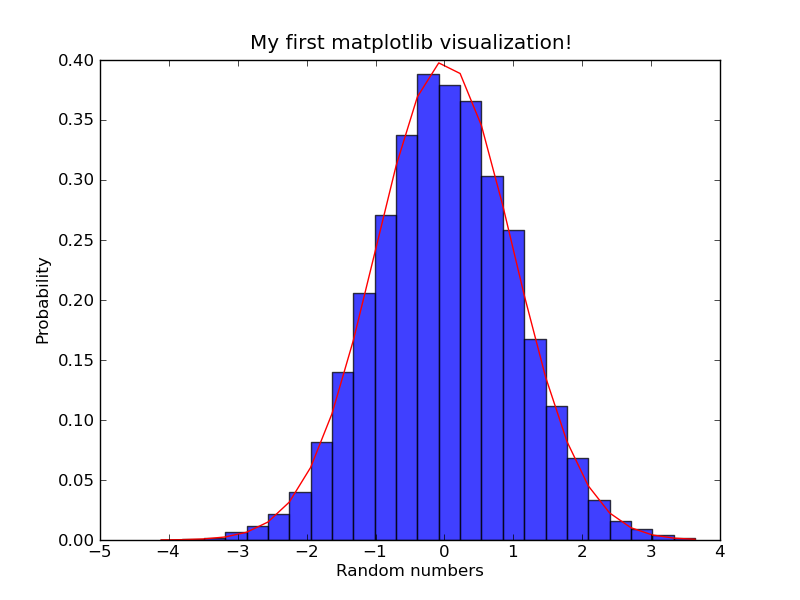
\includegraphics[width=10cm]{matplotlib_first.png}
    \end{center}
\end{frame}

\begin{frame}[fragile]
    \frametitle{My first \texttt{ggplot2} visualization 1/4}
    Again, first load library and create data
    \begin{block}{Load the \texttt{ggplot2} package}
        \begin{lstlisting}[language=R]
> library(ggplot2)
        \end{lstlisting}
    \end{block}
    \begin{block}{Create our first \texttt{data.frame}}
        \begin{lstlisting}[language=R]
> random.numbers<-rnorm(10000,0,1)
> norm.dframe<-as.data.frame(list(Norm=random.numbers))
        \end{lstlisting}
    \end{block}
    \begin{block}{Create base \texttt{ggplot2} layer}
        \begin{lstlisting}[language=R]
> norm.plt<-ggplot(norm.dframe,aes(Norm)) + 
    geom_histogram(aes(y = ..density.., fill="blue", 
    colour="black",alpha=0.75))
        \end{lstlisting}
    \end{block}
\end{frame}

\begin{frame}[fragile]
    \frametitle{My first \texttt{ggplot2} visualization 2/4}
    Next, we build up layers from the base
    \begin{block}{Add Normal PDF}
        \begin{lstlisting}[language=R]
> norm.plt<-norm.plt+stat_function(fun = dnorm, 
        colour = "red")
        \end{lstlisting}
    \end{block} 
    \begin{block}{Deal with colors and legends}
        \begin{lstlisting}[language=R]
> norm.plt<-norm.plt+scale_colour_manual(values = 
        c("black"="black","red"="red"), legend = FALSE)
> norm.plt<-norm.plt+scale_fill_manual(values = 
    c("blue"="blue"), legend = FALSE) 
> norm.plt<-norm.plt+scale_alpha(legend = FALSE)+
        \end{lstlisting}
    \end{block}
\end{frame}

\begin{frame}[fragile]
    \frametitle{My first \texttt{ggplot2} visualization 3/4}
    Finally, add add labels and save
    \begin{block}{This time, we'll make a PDF}
        \begin{lstlisting}[language=R]
> norm.plt<-norm.plt+xlab("Random numbers")
> norm.plt<-norm.plt+ylab("Density")
> norm.plt<-norm.plt+opts(title=
        "My first ggplot2 visualization!")
> ggsave(plot = norm.plt, filename = 
    "ggplot2_first.pdf", height = 6, 
    width = 8)
        \end{lstlisting}
    \end{block}
\end{frame}

\begin{frame}[fragile]
    \frametitle{My first \texttt{ggplot2} visualization 4/4}
    Who's the baddest data visualizer?! You are!
    \begin{center}
        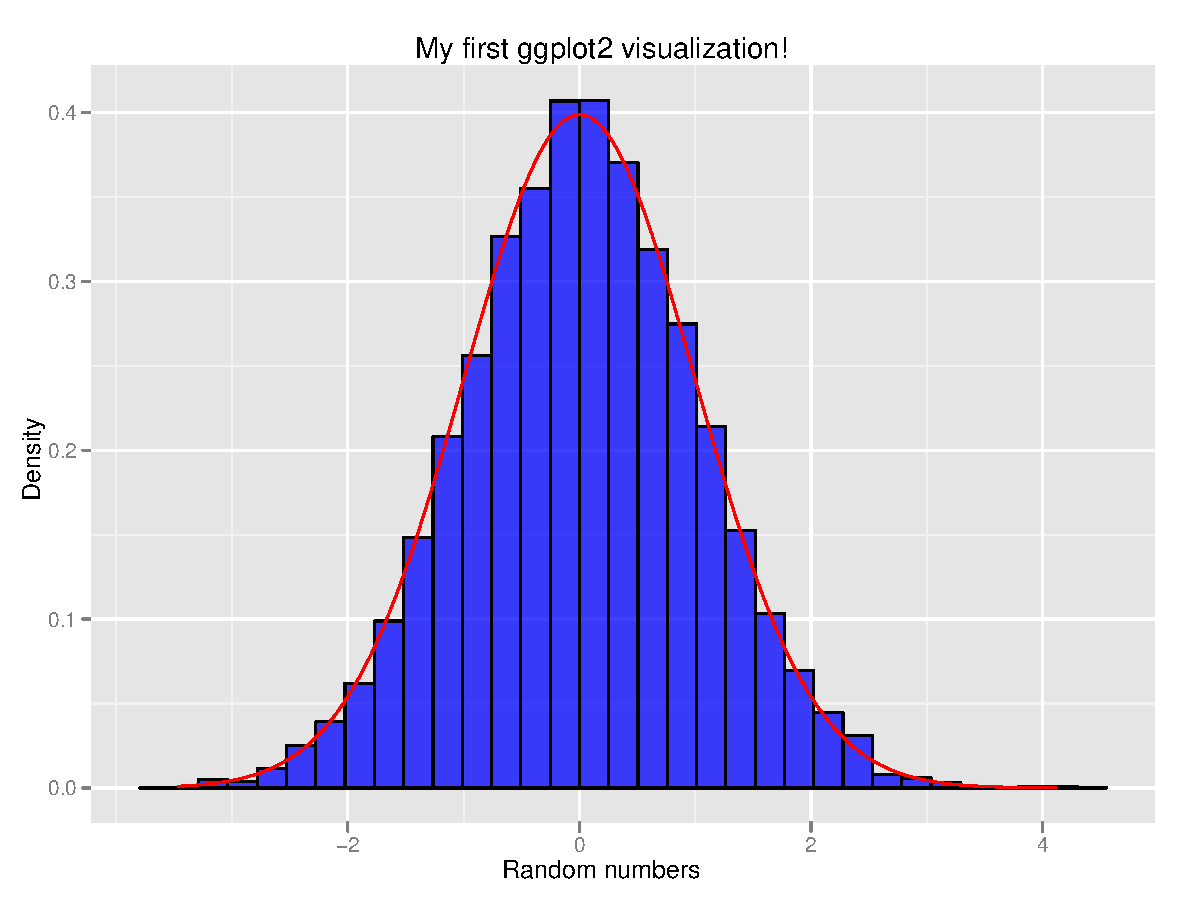
\includegraphics[width=10cm]{ggplot2_first.pdf}
    \end{center}
\end{frame}

% subsection my_first_visualization (end)

% section visualization (end)


\end{document}
